\chapter{Exploratory analysis of the corpora and lexicons}
\label{sec:eda}

This section describes the data the system signs from, before any result is reported: how large each corpus is,
which words dominate it, how much of it each lexicon can sign, and which sources supply the signs.

\section{The corpora}
Table~\ref{tab:eda_corpora} compares the four corpora. All share the same 6,236 verses; the hadith sets differ because
not every hadith of the encyclopedia is translated into every language. The hadith make up most of the text (80--89\% of
tokens), since each carries a title and a scholarly explanation. The Arabic corpus has more than four times the distinct
words of the English one (62,613 against 13,612) for fewer tokens, because Arabic writes conjunctions, prepositions and
pronouns as part of the word; Turkish, an agglutinative language, shows the same effect (49,131 distinct words). Lexicon
matching therefore has to reduce words to their stems (Section~\ref{sec:glossing}), and distinct-word coverage is a poor
guide for these two languages; occurrence coverage is the figure we report.

\begin{table}[ht]
\centering\small
\caption{The four knowledge corpora: size, and the share of content-word occurrences that the sign lexicon of
each mode can sign. Urdu answers are signed with Indian Sign Language, whose glosses are English words, so its
coverage is measured on the English corpus of the same verses and hadith.}
\label{tab:eda_corpora}
\begin{tabular}{l r r r r r r}
\toprule
Mode & Passages & Tokens & Distinct words & Content tokens & Qur'an covered & Hadith covered \\
\midrule
English / ASL & 8,564 & 865,157 & 13,612 & 425,556 & 84.4\% & 80.3\% \\
Arabic / ArSL & 9,810 & 727,335 & 62,613 & 595,022 & 46.3\% & 54.1\% \\
Turkish / T\.{I}D & 8,386 & 606,797 & 49,131 & 498,831 & 15.8\% & 16.0\% \\
Urdu / ISL & 8,456 & 942,554 & 18,035 & 569,880 & 54.4\% & 50.4\% \\
\bottomrule
\end{tabular}
\end{table}

\begin{table}[ht]
\centering\small
\caption{The ten most frequent content words of the Qur'an and of the hadith in each corpus (tokens of two
letters or fewer, mostly clitic fragments, are not shown). $^\dagger$: no sign in that mode's lexicon.}
\label{tab:eda_top}
\begin{tabularx}{\textwidth}{l l Y}
\toprule
Corpus & Part & Most frequent content words \\
\midrule
English & Qur'an & allah (2,976), not (2,194), indeed (1,498), lord (972), said (821), say (767), people (740), upon (627), day (500), among (474) \\
 & Hadith & allah (20,607), upon (8,496), peace (7,724), blessings (7,539), said (6,828), prophet (5,704), not (5,130), one (3,808), messenger (3,694), pleased (3,499) \\
\addlinespace
Arabic & Qur'an & \ar{الله} (2,155), \ar{الا}$^\dagger$ (763), \ar{ولا}$^\dagger$ (658), \ar{قال} (416), \ar{لهم} (373), \ar{لكم} (337), \ar{وان} (323), \ar{بما} (296), \ar{الارض} (287), \ar{امنوا} (263) \\
 & Hadith & \ar{الله} (31,590), \ar{عليه} (15,902), \ar{صلي} (12,894), \ar{وسلم}$^\dagger$ (12,493), \ar{قال} (9,013), \ar{النبي} (6,583), \ar{رسول} (5,569), \ar{رضي} (4,952), \ar{فقال}$^\dagger$ (3,831), \ar{عنه}$^\dagger$ (3,709) \\
\addlinespace
Turkish & Qur'an & allah$^\dagger$ (3,092), iman (602), size (589), onların (569), onlara$^\dagger$ (566), şüphesiz (565), işte (500), eğer$^\dagger$ (470), onu$^\dagger$ (451), onları (446) \\
 & Hadith & aleyhi$^\dagger$ (8,394), sallallahu (8,345), sellem$^\dagger$ (8,319), allah$^\dagger$ (7,514), radıyallahu$^\dagger$ (4,171), şöyle$^\dagger$ (4,050), rasûlullah$^\dagger$ (3,673), anh$^\dagger$ (2,820), dedi$^\dagger$ (2,454), nebi$^\dagger$ (2,269) \\
\addlinespace
Urdu & Qur'an & \ar{اللہ} (3,121), \ar{تعالی} (1,552), \ar{اپنے} (1,108), \ar{واﻻ} (852), \ar{پھر} (829), \ar{لوگ} (795), \ar{کوئی} (727), \ar{انہیں} (706), \ar{کرتے} (675), \ar{طرف} (642) \\
 & Hadith & \ar{اللہ} (19,536), \ar{رضی} (5,502), \ar{فرمایا} (4,110), \ar{رسول} (3,991), \ar{عنہ} (3,724), \ar{نبی} (3,660), \ar{اسے} (3,332), \ar{اپنے} (3,273), \ar{پھر} (3,024), \ar{کوئی} (2,602) \\
\addlinespace
\bottomrule
\end{tabularx}
\end{table}

\begin{table}[ht]
\centering\small
\caption{The signs used most often when the Qur'an and hadith are signed: the share of all content-word
occurrences that each sign covers.}
\label{tab:eda_signs}
\begin{tabularx}{\textwidth}{l Y}
\toprule
Lexicon & Most used signs (share of content-word occurrences) \\
\midrule
ASL & ALLAH (5.7\%), SAY (2.5\%), UPON (2.1\%), PEACE (1.8\%), BLESSINGS (1.8\%), NOT (1.7\%), PROPHET (1.4\%), ONE (1.0\%), MESSENGER (1.0\%), PLEASE (0.8\%), PEOPLE (0.7\%), REPORT (0.6\%), EXPLANATION (0.6\%), O (0.5\%), MAN (0.5\%) \\
ArSL & \ar{الله} (5.9\%), \ar{على} (3.2\%), \ar{صلى} (2.2\%), \ar{قال} (1.7\%), \ar{أن} (1.5\%), \ar{نبي} (1.2\%), \ar{رسول} (1.1\%), \ar{رضي} (0.9\%), \ar{له} (0.8\%), \ar{شرح} (0.6\%), \ar{فئة} (0.5\%), \ar{أب} (0.5\%), \ar{رجل} (0.5\%), \ar{الصلاة} (0.4\%), \ar{يوم} (0.4\%) \\
\bottomrule
\end{tabularx}
\end{table}


\section{Frequent words}
Table~\ref{tab:eda_top} lists the most frequent content words. Three patterns hold across languages. First, the name of
God (\emph{Allah}, \ar{الله}, \emph{Allah}, \ar{اللہ}) is the most frequent word of every corpus, so a single sign
already covers a large share of the text. Second, the hadith are dominated by the formulas of transmission and respect:
``peace and blessings be upon him'' (\ar{صلى الله عليه وسلم}, \emph{sallallahu aleyhi ve sellem}, \ar{ﷺ}), ``may Allah be
pleased with him'' (\ar{رضي الله عنه}, \emph{rad\i{}yallahu anh}), and verbs of narration (\emph{said, reported};
\ar{قال}; \emph{dedi, rivayet}). In sign language these formulas are signed as fixed units, not word by word, so they are
the cheapest gaps to close. Third, the Qur'an's frequent words are its theological vocabulary (\emph{Lord, day, people,
believe}; \ar{الأرض، آمنوا}), which overlaps with general dictionaries more than the vocabulary of the hadith
explanations does.

\section{How much each lexicon can sign}
Figure~\ref{fig:covlang} shows the share of content-word occurrences that each mode can sign today. English/ASL is the
most complete (64\% of the Qur'an, 63\% of the hadith), followed by Arabic/ArSL (46\% and 54\%). The Arabic Qur'an is
harder than the Arabic hadith because classical Qur'anic forms are rarer in dictionaries; the Qur'an-curriculum signs
partly offset this.

\paragraph{Turkish.} The T\.{I}D lexicon is still being extracted: 1,308 of the 5,017 dictionary clips have been
converted (980 single-word glosses), and the Islamic-terms channel has not been processed yet. It covers 16\% of
content-word occurrences, and its most frequent gaps are exactly the religious words: \emph{Allah, aleyhi, sellem,
rad\i{}yallahu, ras\^{u}lullah, nebi} (prophet), \emph{rivayet} (narration). A general dictionary does not contain the
vocabulary of religious texts, which is why the Islamic-terms source matters more than its 589 clips suggest.

\paragraph{Urdu.} The Indian Sign Language lexicons (5,181 single-word glosses) cover 51\% of content-word occurrences
of the same texts, measured on the English glosses. Their gaps show the same pattern: \emph{peace, blessings, prophet,
prayer, Lord} have no ISL sign in these general-purpose datasets, so the Urdu mode cannot sign a basic answer until
Islamic terms are added.

\begin{figure}[ht]
\centering
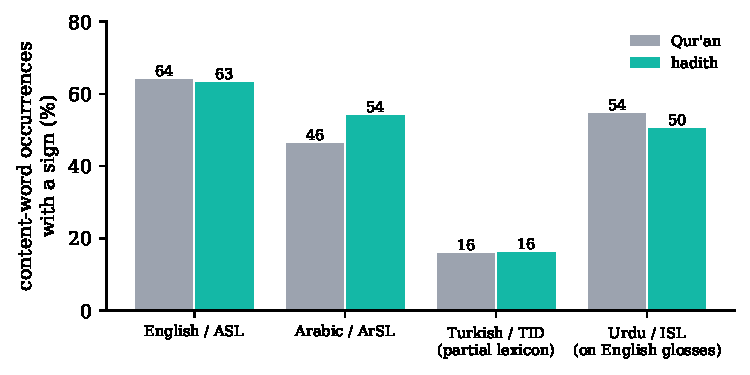
\includegraphics[width=0.72\textwidth]{figures/coverage_languages.pdf}
\caption{Content-word occurrences of the Qur'an and hadith that each mode's lexicon can sign.}
\label{fig:covlang}
\end{figure}

\section{Which sources supply the signs}
Figure~\ref{fig:attribution} attributes every covered occurrence to the source of the sign the matcher returns. In
English, ASL Citizen supplies 40.5\% of the content-word occurrences through 1,234 different signs, while the 40 GDM
Islamic signs supply 10.2\%: forty religious signs do a quarter of the work of a 2,204-sign general dictionary. In Arabic
the effect is stronger: the 324 signs cut from the Qur'an curriculum cover 28.8\% of all content-word occurrences, more
than KArSL, the unified dictionary and the Kuwaiti dictionary together (22.3\%). Dictionaries of everyday vocabulary
(children's, scouts', Levantine) contribute below 1\% each. Table~\ref{tab:eda_signs} lists the individual signs used
most: \ar{الله} alone signs 5.9\% of all Arabic content-word occurrences (ALLAH: 5.7\% in English), followed by
\ar{على}, \ar{صلى} and \ar{قال}, which come from the hadith formulas. Two
conclusions follow for collecting data: a small set of religious signs recorded by Deaf signers is worth more than a large
general dictionary, and the hadith formulas should be recorded as phrase signs.

\begin{figure}[ht]
\centering
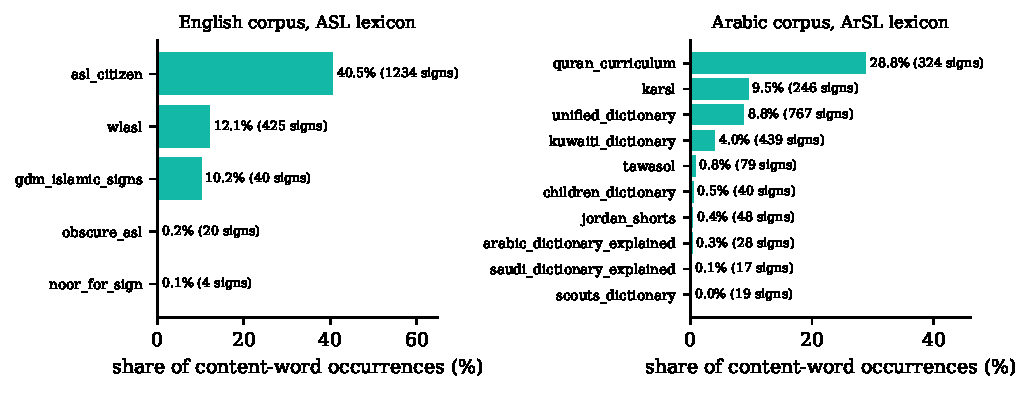
\includegraphics[width=\textwidth]{figures/source_attribution.pdf}
\caption{Share of the corpus's content-word occurrences signed by each lexicon source (in brackets, the number of that
source's signs that are used).}
\label{fig:attribution}
\end{figure}
